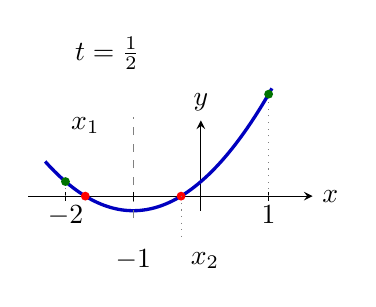
\begin{tikzpicture}[x=.86cm,y=.37cm,>=stealth]
 \draw[->] (-2.55,0)--(1.65,0) node[right]{$x$};\draw[->] (0,-.5)--(0,2.6) node[above]{$y$};
 \draw[very thick,blue!75!black,domain=-2.3:1.05,samples=75] plot (\x,{(\x+1)*(\x+1)-.5});
 \draw[dashed,gray] (-1,-.76)--(-1,2.7);
 \fill[red] (-1.7071,0) circle(1.6pt) (-.2929,0) circle(1.6pt);
 \node[below] at (-2,0) {$-2$};\node[below] at (-1,-1.5) {$-1$};\node[below] at (1,0) {$1$};
 \node[above] at (-1.7071,1.8) {$x_1$};\node[below right] at (-.2929,-1.6) {$x_2$};
 \foreach \v in {-2,-1,1}\draw (\v,.15)--(\v,-.15);
 \draw[dotted,gray] (-2,0)--(-2,.5) (1,0)--(1,3.5) (-.2929,0)--(-.2929,-1.4);
 \fill[green!45!black] (-2,.5) circle(1.6pt) (1,3.5) circle(1.6pt);
 \node[above right] at (-2,4.0) {$t=\frac12$};
\end{tikzpicture}
